% Options for packages loaded elsewhere
\PassOptionsToPackage{unicode}{hyperref}
\PassOptionsToPackage{hyphens}{url}
\PassOptionsToPackage{dvipsnames,svgnames,x11names}{xcolor}
%
\documentclass[
  letterpaper,
  DIV=11,
  numbers=noendperiod]{scrartcl}

\usepackage{amsmath,amssymb}
\usepackage{iftex}
\ifPDFTeX
  \usepackage[T1]{fontenc}
  \usepackage[utf8]{inputenc}
  \usepackage{textcomp} % provide euro and other symbols
\else % if luatex or xetex
  \usepackage{unicode-math}
  \defaultfontfeatures{Scale=MatchLowercase}
  \defaultfontfeatures[\rmfamily]{Ligatures=TeX,Scale=1}
\fi
\usepackage{lmodern}
\ifPDFTeX\else  
    % xetex/luatex font selection
\fi
% Use upquote if available, for straight quotes in verbatim environments
\IfFileExists{upquote.sty}{\usepackage{upquote}}{}
\IfFileExists{microtype.sty}{% use microtype if available
  \usepackage[]{microtype}
  \UseMicrotypeSet[protrusion]{basicmath} % disable protrusion for tt fonts
}{}
\makeatletter
\@ifundefined{KOMAClassName}{% if non-KOMA class
  \IfFileExists{parskip.sty}{%
    \usepackage{parskip}
  }{% else
    \setlength{\parindent}{0pt}
    \setlength{\parskip}{6pt plus 2pt minus 1pt}}
}{% if KOMA class
  \KOMAoptions{parskip=half}}
\makeatother
\usepackage{xcolor}
\setlength{\emergencystretch}{3em} % prevent overfull lines
\setcounter{secnumdepth}{-\maxdimen} % remove section numbering
% Make \paragraph and \subparagraph free-standing
\makeatletter
\ifx\paragraph\undefined\else
  \let\oldparagraph\paragraph
  \renewcommand{\paragraph}{
    \@ifstar
      \xxxParagraphStar
      \xxxParagraphNoStar
  }
  \newcommand{\xxxParagraphStar}[1]{\oldparagraph*{#1}\mbox{}}
  \newcommand{\xxxParagraphNoStar}[1]{\oldparagraph{#1}\mbox{}}
\fi
\ifx\subparagraph\undefined\else
  \let\oldsubparagraph\subparagraph
  \renewcommand{\subparagraph}{
    \@ifstar
      \xxxSubParagraphStar
      \xxxSubParagraphNoStar
  }
  \newcommand{\xxxSubParagraphStar}[1]{\oldsubparagraph*{#1}\mbox{}}
  \newcommand{\xxxSubParagraphNoStar}[1]{\oldsubparagraph{#1}\mbox{}}
\fi
\makeatother

\usepackage{color}
\usepackage{fancyvrb}
\newcommand{\VerbBar}{|}
\newcommand{\VERB}{\Verb[commandchars=\\\{\}]}
\DefineVerbatimEnvironment{Highlighting}{Verbatim}{commandchars=\\\{\}}
% Add ',fontsize=\small' for more characters per line
\usepackage{framed}
\definecolor{shadecolor}{RGB}{241,243,245}
\newenvironment{Shaded}{\begin{snugshade}}{\end{snugshade}}
\newcommand{\AlertTok}[1]{\textcolor[rgb]{0.68,0.00,0.00}{#1}}
\newcommand{\AnnotationTok}[1]{\textcolor[rgb]{0.37,0.37,0.37}{#1}}
\newcommand{\AttributeTok}[1]{\textcolor[rgb]{0.40,0.45,0.13}{#1}}
\newcommand{\BaseNTok}[1]{\textcolor[rgb]{0.68,0.00,0.00}{#1}}
\newcommand{\BuiltInTok}[1]{\textcolor[rgb]{0.00,0.23,0.31}{#1}}
\newcommand{\CharTok}[1]{\textcolor[rgb]{0.13,0.47,0.30}{#1}}
\newcommand{\CommentTok}[1]{\textcolor[rgb]{0.37,0.37,0.37}{#1}}
\newcommand{\CommentVarTok}[1]{\textcolor[rgb]{0.37,0.37,0.37}{\textit{#1}}}
\newcommand{\ConstantTok}[1]{\textcolor[rgb]{0.56,0.35,0.01}{#1}}
\newcommand{\ControlFlowTok}[1]{\textcolor[rgb]{0.00,0.23,0.31}{\textbf{#1}}}
\newcommand{\DataTypeTok}[1]{\textcolor[rgb]{0.68,0.00,0.00}{#1}}
\newcommand{\DecValTok}[1]{\textcolor[rgb]{0.68,0.00,0.00}{#1}}
\newcommand{\DocumentationTok}[1]{\textcolor[rgb]{0.37,0.37,0.37}{\textit{#1}}}
\newcommand{\ErrorTok}[1]{\textcolor[rgb]{0.68,0.00,0.00}{#1}}
\newcommand{\ExtensionTok}[1]{\textcolor[rgb]{0.00,0.23,0.31}{#1}}
\newcommand{\FloatTok}[1]{\textcolor[rgb]{0.68,0.00,0.00}{#1}}
\newcommand{\FunctionTok}[1]{\textcolor[rgb]{0.28,0.35,0.67}{#1}}
\newcommand{\ImportTok}[1]{\textcolor[rgb]{0.00,0.46,0.62}{#1}}
\newcommand{\InformationTok}[1]{\textcolor[rgb]{0.37,0.37,0.37}{#1}}
\newcommand{\KeywordTok}[1]{\textcolor[rgb]{0.00,0.23,0.31}{\textbf{#1}}}
\newcommand{\NormalTok}[1]{\textcolor[rgb]{0.00,0.23,0.31}{#1}}
\newcommand{\OperatorTok}[1]{\textcolor[rgb]{0.37,0.37,0.37}{#1}}
\newcommand{\OtherTok}[1]{\textcolor[rgb]{0.00,0.23,0.31}{#1}}
\newcommand{\PreprocessorTok}[1]{\textcolor[rgb]{0.68,0.00,0.00}{#1}}
\newcommand{\RegionMarkerTok}[1]{\textcolor[rgb]{0.00,0.23,0.31}{#1}}
\newcommand{\SpecialCharTok}[1]{\textcolor[rgb]{0.37,0.37,0.37}{#1}}
\newcommand{\SpecialStringTok}[1]{\textcolor[rgb]{0.13,0.47,0.30}{#1}}
\newcommand{\StringTok}[1]{\textcolor[rgb]{0.13,0.47,0.30}{#1}}
\newcommand{\VariableTok}[1]{\textcolor[rgb]{0.07,0.07,0.07}{#1}}
\newcommand{\VerbatimStringTok}[1]{\textcolor[rgb]{0.13,0.47,0.30}{#1}}
\newcommand{\WarningTok}[1]{\textcolor[rgb]{0.37,0.37,0.37}{\textit{#1}}}

\providecommand{\tightlist}{%
  \setlength{\itemsep}{0pt}\setlength{\parskip}{0pt}}\usepackage{longtable,booktabs,array}
\usepackage{calc} % for calculating minipage widths
% Correct order of tables after \paragraph or \subparagraph
\usepackage{etoolbox}
\makeatletter
\patchcmd\longtable{\par}{\if@noskipsec\mbox{}\fi\par}{}{}
\makeatother
% Allow footnotes in longtable head/foot
\IfFileExists{footnotehyper.sty}{\usepackage{footnotehyper}}{\usepackage{footnote}}
\makesavenoteenv{longtable}
\usepackage{graphicx}
\makeatletter
\newsavebox\pandoc@box
\newcommand*\pandocbounded[1]{% scales image to fit in text height/width
  \sbox\pandoc@box{#1}%
  \Gscale@div\@tempa{\textheight}{\dimexpr\ht\pandoc@box+\dp\pandoc@box\relax}%
  \Gscale@div\@tempb{\linewidth}{\wd\pandoc@box}%
  \ifdim\@tempb\p@<\@tempa\p@\let\@tempa\@tempb\fi% select the smaller of both
  \ifdim\@tempa\p@<\p@\scalebox{\@tempa}{\usebox\pandoc@box}%
  \else\usebox{\pandoc@box}%
  \fi%
}
% Set default figure placement to htbp
\def\fps@figure{htbp}
\makeatother
% definitions for citeproc citations
\NewDocumentCommand\citeproctext{}{}
\NewDocumentCommand\citeproc{mm}{%
  \begingroup\def\citeproctext{#2}\cite{#1}\endgroup}
\makeatletter
 % allow citations to break across lines
 \let\@cite@ofmt\@firstofone
 % avoid brackets around text for \cite:
 \def\@biblabel#1{}
 \def\@cite#1#2{{#1\if@tempswa , #2\fi}}
\makeatother
\newlength{\cslhangindent}
\setlength{\cslhangindent}{1.5em}
\newlength{\csllabelwidth}
\setlength{\csllabelwidth}{3em}
\newenvironment{CSLReferences}[2] % #1 hanging-indent, #2 entry-spacing
 {\begin{list}{}{%
  \setlength{\itemindent}{0pt}
  \setlength{\leftmargin}{0pt}
  \setlength{\parsep}{0pt}
  % turn on hanging indent if param 1 is 1
  \ifodd #1
   \setlength{\leftmargin}{\cslhangindent}
   \setlength{\itemindent}{-1\cslhangindent}
  \fi
  % set entry spacing
  \setlength{\itemsep}{#2\baselineskip}}}
 {\end{list}}
\usepackage{calc}
\newcommand{\CSLBlock}[1]{\hfill\break\parbox[t]{\linewidth}{\strut\ignorespaces#1\strut}}
\newcommand{\CSLLeftMargin}[1]{\parbox[t]{\csllabelwidth}{\strut#1\strut}}
\newcommand{\CSLRightInline}[1]{\parbox[t]{\linewidth - \csllabelwidth}{\strut#1\strut}}
\newcommand{\CSLIndent}[1]{\hspace{\cslhangindent}#1}

\KOMAoption{captions}{tableheading}
\makeatletter
\@ifpackageloaded{caption}{}{\usepackage{caption}}
\AtBeginDocument{%
\ifdefined\contentsname
  \renewcommand*\contentsname{Table of contents}
\else
  \newcommand\contentsname{Table of contents}
\fi
\ifdefined\listfigurename
  \renewcommand*\listfigurename{List of Figures}
\else
  \newcommand\listfigurename{List of Figures}
\fi
\ifdefined\listtablename
  \renewcommand*\listtablename{List of Tables}
\else
  \newcommand\listtablename{List of Tables}
\fi
\ifdefined\figurename
  \renewcommand*\figurename{Figure}
\else
  \newcommand\figurename{Figure}
\fi
\ifdefined\tablename
  \renewcommand*\tablename{Table}
\else
  \newcommand\tablename{Table}
\fi
}
\@ifpackageloaded{float}{}{\usepackage{float}}
\floatstyle{ruled}
\@ifundefined{c@chapter}{\newfloat{codelisting}{h}{lop}}{\newfloat{codelisting}{h}{lop}[chapter]}
\floatname{codelisting}{Listing}
\newcommand*\listoflistings{\listof{codelisting}{List of Listings}}
\makeatother
\makeatletter
\makeatother
\makeatletter
\@ifpackageloaded{caption}{}{\usepackage{caption}}
\@ifpackageloaded{subcaption}{}{\usepackage{subcaption}}
\makeatother

\usepackage{bookmark}

\IfFileExists{xurl.sty}{\usepackage{xurl}}{} % add URL line breaks if available
\urlstyle{same} % disable monospaced font for URLs
\hypersetup{
  pdftitle={Financial Report on the Clorox Company (CLX)},
  pdfkeywords={Financial Report, Feduciary, Course Project},
  colorlinks=true,
  linkcolor={blue},
  filecolor={Maroon},
  citecolor={Blue},
  urlcolor={Blue},
  pdfcreator={LaTeX via pandoc}}


\title{Financial Report on the Clorox Company (CLX)}
\usepackage{etoolbox}
\makeatletter
\providecommand{\subtitle}[1]{% add subtitle to \maketitle
  \apptocmd{\@title}{\par {\large #1 \par}}{}{}
}
\makeatother
\subtitle{A Project for the Computational Finance Course}
\author{Andrey Malyukov \and Roza Bass}
\date{}

\begin{document}
\maketitle
\begin{abstract}
In this Project for the Computational Finance course led by prof. Alan
Solomon at the Sami Shamoon College of Engineering, we aim to
demonstrate basic understanding of the course material by writing a
guide for the feduciary on how to provide guidance for investors using
the tools of computational finance.
\end{abstract}

\renewcommand*\contentsname{Table of contents}
{
\hypersetup{linkcolor=}
\setcounter{tocdepth}{3}
\tableofcontents
}

\section{}\label{section}

\begin{quote}
\textbf{On the simplified nature of analysis in this document.}

Subject of financial analysis is very information-dense and to perform
such an analysis (be it an analysis of industrial sectors, fundamental,
technical, etc.) in earnest is a non-trivial job that we don't see
ourselves capable of performing.

Therefore, this document aims to provide a simplified, non-rigorous
analysis aiming to showcase our understanding of course material and
minimal proficiency in scientific communication using tools such as web
scraping and searching for financial data, DeepSeek LLM with Web Search
functionality, R language {[}{``R: {The R Project} for {Statistical
Computing}''} (n.d.){]}, its ``tidyquant'' package {[}Dancho and Vaughan
(2025){]} and Quarto scientific publishing system {[}{``Quarto''}
(n.d.){]}.
\end{quote}

\subsection{Sector Analysis}\label{sector-analysis}

\section{}\label{section-1}

\begin{quote}
\textbf{Note}

In this section we analyze financial data on websites such as
\url{https://finance.yahoo.com}, as well as using the
\href{https://chat.deepseek.com/}{DeepSeek LLM} to find analysis on the
web and provide summaries. Some basic charting using R language {[}{``R:
{The R Project} for {Statistical Computing}''} (n.d.){]} is introduced.
\end{quote}

\subsubsection{Financial Analysis of the Clorox Company in the Consumer
Defensive
Sector}\label{financial-analysis-of-the-clorox-company-in-the-consumer-defensive-sector}

\paragraph{\texorpdfstring{\textbf{1. Sector
Analysis}}{1. Sector Analysis}}\label{sector-analysis-1}

Clorox operates in the \textbf{Consumer Defensive sector}, specifically
within the Household and Personal Products sub-sector. This sector is
characterized by stable demand and recession resilience.

Sector's \textbf{Market Cap} is estimated to be \$3.7 trillion. The
\textbf{Market Weight (Share)} of the sector relative to the other 10
sectors is 5.45\%.

Sector's \textbf{Year-To-Date Return} is 6.17\%, which outperforms
S\&P500 (3.54\%).

\begin{center}\rule{0.5\linewidth}{0.5pt}\end{center}

\paragraph{\texorpdfstring{\textbf{2. Position Relative to
Competitors}}{2. Position Relative to Competitors}}\label{position-relative-to-competitors}

Clorox's market share inside it's sector is relatively small:

\begin{longtable}[]{@{}
  >{\raggedright\arraybackslash}p{(\linewidth - 8\tabcolsep) * \real{0.2192}}
  >{\raggedright\arraybackslash}p{(\linewidth - 8\tabcolsep) * \real{0.2329}}
  >{\raggedright\arraybackslash}p{(\linewidth - 8\tabcolsep) * \real{0.2329}}
  >{\raggedright\arraybackslash}p{(\linewidth - 8\tabcolsep) * \real{0.1644}}
  >{\raggedright\arraybackslash}p{(\linewidth - 8\tabcolsep) * \real{0.1507}}@{}}
\toprule\noalign{}
\begin{minipage}[b]{\linewidth}\raggedright
COMPANY NAME
\end{minipage} & \begin{minipage}[b]{\linewidth}\raggedright
MARKET SHARE 12 Months Ending Q4 2024
\end{minipage} & \begin{minipage}[b]{\linewidth}\raggedright
MARKET SHARE 12 Months Ending Q3 2024
\end{minipage} & \begin{minipage}[b]{\linewidth}\raggedright
MARKET SHARE MRQ Q4 2024
\end{minipage} & \begin{minipage}[b]{\linewidth}\raggedright
MARKET SHARE Q3 2024
\end{minipage} \\
\midrule\noalign{}
\endhead
\bottomrule\noalign{}
\endlastfoot
\textbf{The Clorox Company} & 2.61\% & 2.80\% & 2.42 \% & 2.66 \% \\
The Campbells Company & 3.60\% & 3.61\% & 3.97\% & 3.46\% \\
Colgate palmolive Company & 7.32\% & 7.54\% & 7.09\% & 7.59\% \\
Conagra Brands Inc & 4.58\% & 4.61\% & 4.58\% & 4.21\% \\
Ecolab Inc & 5.06\% & 5.07\% & 5.26\% & 5.40\% \\
Mccormick and Company Incorporated & 2.45\% & 2.50\% & 2.58\% &
2.53\% \\
Procter and Gamble Co & 30.72\% & 31.46\% & 31.37\% & 32.77\% \\
Hormel Foods Corporation & 5.52\% & 5.65\% & 5.09\% & 4.37\% \\
Avon Products Inc & 1.15\% & 1.28\% & 0.95\% & 1.23\% \\
Horizon Kinetics Holding Corporation & 0.01\% & 0.00\% & 0.02\% &
0.00\% \\
Ingredion Incorporated & 2.75\% & 2.89\% & 2.68\% & 2.83\% \\
Lancaster Colony Corporation & 0.69\% & 0.70\% & 0.73\% & 0.70\% \\
J and j Snack Foods Corp & 0.58\% & 0.59\% & 0.52\% & 0.64\% \\
Treehouse Foods Inc & 1.19\% & 1.24\% & 1.20\% & 1.19\% \\
Dole Plc & 3.00\% & 3.46\% & 3.00\% & 3.46\% \\
Church and Dwight Co Inc & 2.22\% & 2.27\% & 2.27\% & 2.28\% \\
Coty Inc & 2.22\% & 2.30\% & 2.39\% & 2.52\% \\
Unilever Plc & 24.32\% & 22.02\% & 24.32\% & 22.02\% \\
SUBTOTAL & 100\% & 100\% & 100\% & 100\% \\
\end{longtable}

CLX's Market share relative to its competitors, as of Q4 2024 within the
Consumer Non Cyclical Sector (i.e.~Consumer Defensive), source: {``The
{Clorox Market} Share Relative to Its Competitors, as of {Q4} 2024 -
{CSIMarket}''} (n.d.)

Clorox competes with major players such as \textbf{Procter \& Gamble
(PG)}, \textbf{Colgate-Palmolive (CL)}, \textbf{Church \& Dwight (CHD)},
and \textbf{Kimberly-Clark (KMB)}. Let's look at their stock price
relative to each other using R language.

\pandocbounded{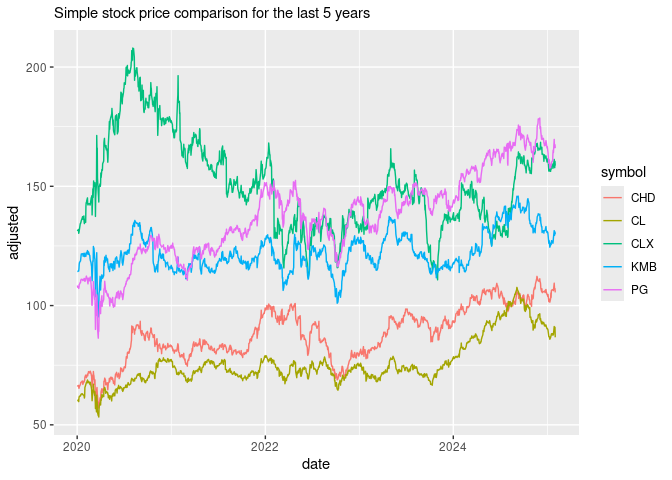
\includegraphics[keepaspectratio]{index_files/figure-latex/notebooks-sector-cell-2-output-2.png}}

\subsubsection{\texorpdfstring{\textbf{Conclusion}}{Conclusion}}\label{conclusion}

We can use web scraping, modern LLM chatbots and R language to perform
all the necessary analysis of the particular industrial sector and the
corporation's position in this sector. The analysis shows small, but
strong position of the company relative to it's sector, as well
characterizes the sector itself.

\subsection{Personality of the
Company}\label{personality-of-the-company}

\section{}\label{section-2}

\begin{quote}
\textbf{Note}

In this section we collect and cite a variety of publicly available
sources to perform an analysis of the company personality. We use use
DeepSeek LLM with Web Search functionality to collect and analyze these
sources.
\end{quote}

\paragraph{\texorpdfstring{\textbf{Company Purpose and
Responsibility}}{Company Purpose and Responsibility}}\label{company-purpose-and-responsibility}

\subparagraph{\texorpdfstring{\textbf{Company
Purpose}}{Company Purpose}}\label{company-purpose}

Clorox's stated purpose is to ``champion people to be well and thrive
every single day'' {[}{``Purpose \& {Values}''} (n.d.){]}. As a health
and wellness company, Clorox aims to make a meaningful and positive
impact on the world by improving the health and safety of employees,
consumers, and communities. All of this is reflected in their
family-friendly and inclusive branding.

\subparagraph{\texorpdfstring{\textbf{Responsibility
Policies}}{Responsibility Policies}}\label{responsibility-policies}

Clorox integrates environmental, social, and governance (ESG) goals into
its core business strategy {[}{``Responsibility''} (n.d.){]}. Key areas
of focus include:

\begin{itemize}
\tightlist
\item
  \textbf{Healthy Lives}: Promoting employee well-being, product
  stewardship, and transparency in ingredients.\\
\item
  \textbf{Clean World}: Reducing greenhouse gas emissions, plastic
  waste, and transitioning to 100\% renewable energy in U.S. and Canada
  operations.\\
\item
  \textbf{Thriving Communities}: Ensuring pay equity, fostering
  diversity, and supporting community initiatives.
\end{itemize}

Clorox has set ambitious targets, such as achieving net-zero emissions
by 2050.

\subparagraph{\texorpdfstring{\textbf{IGNITE
Strategy}}{IGNITE Strategy}}\label{ignite-strategy}

The IGNITE strategy is Clorox's long-term plan to drive what the company
calls a ``purpose-driven growth'' {[}{``{IGNITE Strategy}''} (n.d.){]}
by aligning financial goals with ESG priorities. Key pillars include:

\begin{itemize}
\tightlist
\item
  \textbf{Fuel Growth}: Leveraging technology and sustainability to
  generate cost savings and reinvest in brands.\\
\item
  \textbf{Innovate Experiences}: Building purpose-driven brands and
  enhancing consumer experiences through personalized and sustainable
  products.\\
\item
  \textbf{Reimagine Work}: Creating an inclusive workplace and
  simplifying operations to drive efficiency.\\
\item
  \textbf{Evolve Portfolio}: Expanding into consumer megatrends like
  sustainability and wellness.
\end{itemize}

The strategy also includes specific financial targets, such as 2-4\% net
sales growth and 11-13\% free cash flow generation.

\paragraph{\texorpdfstring{\textbf{Key Executives, Their Commitment and
Performance}}{Key Executives, Their Commitment and Performance}}\label{key-executives-their-commitment-and-performance}

\begin{longtable}[]{@{}
  >{\raggedright\arraybackslash}p{(\linewidth - 6\tabcolsep) * \real{0.2432}}
  >{\raggedright\arraybackslash}p{(\linewidth - 6\tabcolsep) * \real{0.5405}}
  >{\raggedright\arraybackslash}p{(\linewidth - 6\tabcolsep) * \real{0.0946}}
  >{\raggedright\arraybackslash}p{(\linewidth - 6\tabcolsep) * \real{0.1216}}@{}}
\toprule\noalign{}
\begin{minipage}[b]{\linewidth}\raggedright
Name
\end{minipage} & \begin{minipage}[b]{\linewidth}\raggedright
Title
\end{minipage} & \begin{minipage}[b]{\linewidth}\raggedright
Pay
\end{minipage} & \begin{minipage}[b]{\linewidth}\raggedright
Year Born
\end{minipage} \\
\midrule\noalign{}
\endhead
\bottomrule\noalign{}
\endlastfoot
Ms.~Linda J. Rendle & CEO \& Chairman & 3.93M & 1979 \\
Mr.~Kevin B. Jacobsen & Executive VP \& CFO & 1.91M & 1967 \\
Mr.~Eric H. Reynolds & Executive VP and Chief Operating \& Strategy
Officer & 1.96M & 1970 \\
Ms.~Angela C. Hilt & Executive VP, Chief Legal Officer \& Corporate
Secretary & 1.45M & 1972 \\
Ms.~Kirsten M. Marriner & Executive VP and Chief People \& Corporate
Affairs Officer & 1.54M & 1973 \\
Ms.~Laura E. Peck & VP, Chief Accounting Officer \& Corporate Controller
& -- & 1977 \\
Ms.~Chau Banks & Senior VP and Chief Information \& Data Officer & -- &
1970 \\
Ms.~Lisah Burhan & Vice President of Investor Relations & -- & -- \\
Mr.~Eric Sean Schwartz & Senior VP \& Chief Marketing Officer & -- &
1972 \\
Mr.~Erbie L. Foster Jr. & Chief Diversity Officer & -- & -- \\
\end{longtable}

Key Executives, source: {[}{``The {Clorox Company} ({CLX}) {Company
Profile} \& {Facts}''} (n.d.){]}

According to {[}{``The {Clorox Company}: {Business Model}, {SWOT
Analysis}, and {Competitors} 2024 - {PitchGrade}''} (n.d.){]}, CEO and
Chairman Linda J. Rendle, as well as the other executives and board
members have significant ownership stakes at the company, indicating
high confidence in their business.

Financial analysis website Simply WallSt gives the upper management team
at Clorox high marks on all 4 criteria: Compensation vs Market,
Compensation vs Earnings, Experienced Management and Experienced Board
{[}{``The {Clorox Company} ({CLX}) {Leadership} \& {Management Team
Analysis}''} (n.d.){]}.

\paragraph{\texorpdfstring{\textbf{Company Brand and
Reputation}}{Company Brand and Reputation}}\label{company-brand-and-reputation}

Clorox is a globally recognized leader in the cleaning and consumer
products industry, known for its trusted brands such as \textbf{Clorox
Bleach}, \textbf{Pine-Sol}, \textbf{Hidden Valley}, \textbf{Brita}, and
\textbf{Burt's Bees}.

The company has received numerous accolades, including being named one
of \textbf{America's Greenest Companies} by Newsweek, a \textbf{Safer
Choice Partner of the Year} by the EPA, and a top performer in the
\textbf{Human Rights Campaign Foundation's Corporate Equality Index}.
Its sustainable brands, such as \textbf{Brita}, \textbf{Burt's Bees},
and \textbf{Green Works}, have gained significant consumer trust for
their eco-friendly and socially responsible practices
{[}{``Recognitions''} (n.d.){]}.

\begin{center}\rule{0.5\linewidth}{0.5pt}\end{center}

In August 2023, Clorox experienced a severe \textbf{cyberattack}
{[}Mascellino (2023){]} that disrupted its IT systems and operations.
The attack, which was detected on August 14, forced the company to take
affected systems offline, leading to significant production delays and
supply chain disruptions. Clorox activated its business continuity
plans, reverting to manual processes for order fulfillment and customer
communications.

The cyberattack had a material financial impact, with Clorox reporting a
23-28\% decline in quarterly sales and a drop in its stock price by over
25\% following the incident.

Clorox's response to the cyberattack highlighted its crisis management
capabilities. The company maintained transparency by providing regular
updates to stakeholders and implementing phased recovery plans to
restore operations safely. Brand and reputation were not severely
damaged in the process.

\paragraph{\texorpdfstring{\textbf{Conclusion}}{Conclusion}}\label{conclusion-1}

We can use modern LLM chatbots to collect publicly available sources and
perform analysis of the company personality. The analysis shows strong
branding, good leadership and consistent performance.

\subsection{Fundamental Analysis}\label{fundamental-analysis}

\section{}\label{section-3}

\begin{quote}
\textbf{Note}

In this section we will take a look at quantitative fundamental analysis
tools provided by the ``tidyquant'' R language package {[}Dancho and
Vaughan (2025){]} and use them to get key financial ratios of
fundamental analysis for the Clorox company. This section is based on
the following wonderful tutorial: {``Performance {Analysis} with
Tidyquant''} (n.d.)
\end{quote}

\paragraph{\texorpdfstring{\textbf{Basic Fundamental Analysis of the
Clorox
Company}}{Basic Fundamental Analysis of the Clorox Company}}\label{basic-fundamental-analysis-of-the-clorox-company}

First let's retrieve 5-year period returns from the prices adjusted for
stock splits, both for Clorox and S\&P500 as the baseline. Next, we
combine both datasets (Clorox and S\&P500 returns) using ``left-join''
on the ``date'' field. Using this dataset, we can retrieve all kind of
fundamental metrics, such as \textbf{Alpha} (0.0008), \textbf{Beta}
(0.414).

\begin{Shaded}
\begin{Highlighting}[]
\NormalTok{library(tidyverse)}
\end{Highlighting}
\end{Shaded}

\begin{verbatim}
# A tibble: 1 × 3
# Groups:   symbol [1]
  symbol  Alpha  Beta
  <chr>   <dbl> <dbl>
1 CLX    0.0008 0.414
\end{verbatim}

We can also get the \textbf{Annualized Sharpe Ratio and Returns},
\textbf{Types of Mean Return (Geometric, Arithmetic, etc.)},
\textbf{Kurtosis}, as well as \textbf{Maximum and Median Return} by
following the similar steps (no need for the baseline this time).

\begin{Shaded}
\begin{Highlighting}[]
\NormalTok{library(tidyverse)}
\NormalTok{library(tidyquant)}

\NormalTok{Ra }\OperatorTok{\textless{}{-}} \StringTok{"CLX"} \OperatorTok{|\textgreater{}}
\NormalTok{    tq\_get(get  }\OperatorTok{=} \StringTok{"stock.prices"}\NormalTok{,}
           \ImportTok{from} \OperatorTok{=} \StringTok{"2020{-}01{-}01"}\NormalTok{,}
\NormalTok{           to   }\OperatorTok{=} \StringTok{"2025{-}02{-}01"}\NormalTok{) }\OperatorTok{|\textgreater{}}
\NormalTok{    group\_by(symbol) }\OperatorTok{|\textgreater{}}
\NormalTok{    tq\_transmute(select     }\OperatorTok{=}\NormalTok{ adjusted, }
\NormalTok{                 mutate\_fun }\OperatorTok{=}\NormalTok{ periodReturn, }
\NormalTok{                 period     }\OperatorTok{=} \StringTok{"monthly"}\NormalTok{, }
\NormalTok{                 col\_rename }\OperatorTok{=} \StringTok{"Ra"}\NormalTok{)}

\NormalTok{Ra }\OperatorTok{|\textgreater{}}
\NormalTok{  tq\_performance(Ra }\OperatorTok{=}\NormalTok{ Ra, Rb }\OperatorTok{=}\NormalTok{ NULL, performance\_fun }\OperatorTok{=}\NormalTok{ table.AnnualizedReturns) }\OperatorTok{|\textgreater{}}
  \BuiltInTok{print}\NormalTok{()}
\end{Highlighting}
\end{Shaded}

\begin{verbatim}
# A tibble: 1 × 4
# Groups:   symbol [1]
  symbol AnnualizedReturn `AnnualizedSharpe(Rf=0%)` AnnualizedStdDev
  <chr>             <dbl>                     <dbl>            <dbl>
1 CLX              0.0381                     0.153            0.249# A tibble: 1 × 17
# Groups:   symbol [1]
  symbol ArithmeticMean GeometricMean Kurtosis `LCLMean(0.95)` Maximum Median
  <chr>           <dbl>         <dbl>    <dbl>           <dbl>   <dbl>  <dbl>
1 CLX            0.0056        0.0031     1.20         -0.0128   0.218 0.0054
# ℹ 10 more variables: Minimum <dbl>, NAs <dbl>, Observations <dbl>,
#   Quartile1 <dbl>, Quartile3 <dbl>, SEMean <dbl>, Skewness <dbl>,
#   Stdev <dbl>, `UCLMean(0.95)` <dbl>, Variance <dbl>
\end{verbatim}

\paragraph{\texorpdfstring{\textbf{Conclusion}}{Conclusion}}\label{conclusion-2}

We can use the ``tidyquant'' R language package to perform fundamental
analysis of the company and obtain all of the key financial ratios for
such analysis. The analysis shows a company in recovery with strong
fundamentals.

\subsection{Technical Analysis}\label{technical-analysis}

\section{}\label{section-4}

\begin{quote}
\textbf{Note}

Technical analysis in this section follows the wonderful tutorial
provided here: {[}{``Financial Modeling with {R}''} (n.d.){]}
\end{quote}

\paragraph{\texorpdfstring{\textbf{Basic Technical Analysis of the
Clorox
Company}}{Basic Technical Analysis of the Clorox Company}}\label{basic-technical-analysis-of-the-clorox-company}

We'll start with providing a simple plot of stock price movement.

\begin{Shaded}
\begin{Highlighting}[]
\NormalTok{library(tidyquant)}
\end{Highlighting}
\end{Shaded}

\pandocbounded{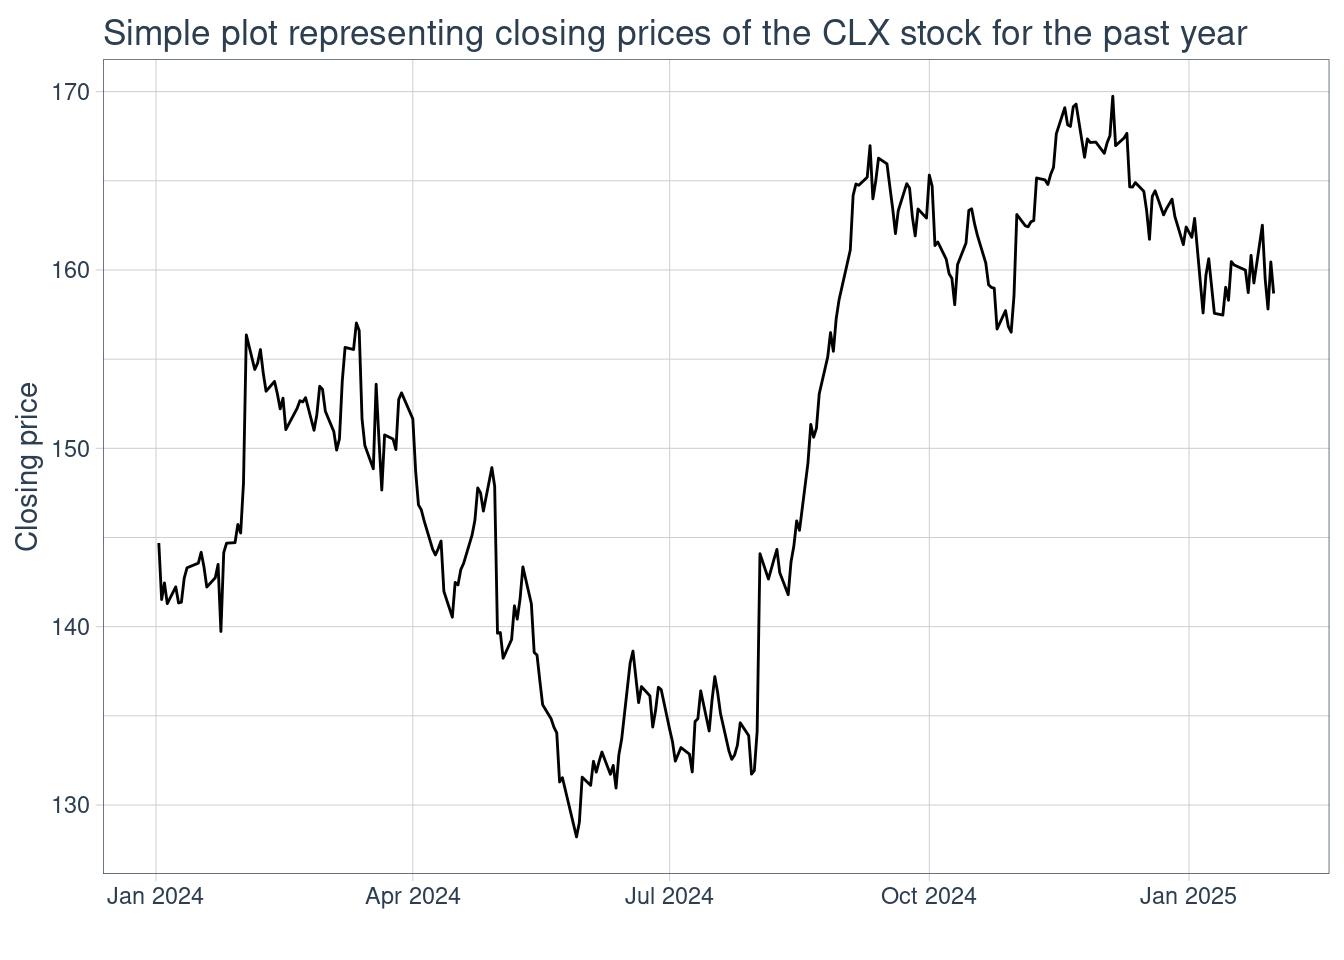
\includegraphics[keepaspectratio]{index_files/figure-latex/notebooks-technical-cell-2-output-2.png}}

To identify basic trend in this movement, we then chart the
\textbf{Simple Moving Average}.

\begin{Shaded}
\begin{Highlighting}[]
\NormalTok{library(tidyquant)}
\NormalTok{library(ggplot2)}
\NormalTok{library(dplyr)}
\NormalTok{CLX }\OperatorTok{\textless{}{-}}\NormalTok{ tq\_get(}\StringTok{"CLX"}\NormalTok{, get }\OperatorTok{=} \StringTok{"stock.prices"}\NormalTok{, }\ImportTok{from} \OperatorTok{=} \StringTok{"2024{-}01{-}01"}\NormalTok{, }
\NormalTok{               to }\OperatorTok{=} \StringTok{"2025{-}02{-}01"}\NormalTok{)}
\NormalTok{CLX }\OperatorTok{|\textgreater{}}
\NormalTok{  ggplot(aes(x }\OperatorTok{=}\NormalTok{ date, y }\OperatorTok{=}\NormalTok{ close)) }\OperatorTok{+}
\NormalTok{    geom\_line()  }\OperatorTok{+}
\NormalTok{    geom\_ma(ma\_fun }\OperatorTok{=}\NormalTok{ SMA, n }\OperatorTok{=} \DecValTok{25}\NormalTok{, linetype }\OperatorTok{=} \DecValTok{1}\NormalTok{, size }\OperatorTok{=} \FloatTok{1.25}\NormalTok{) }\OperatorTok{+}
\NormalTok{    labs(y }\OperatorTok{=} \StringTok{"Closing Price"}\NormalTok{, x }\OperatorTok{=} \StringTok{""}\NormalTok{) }\OperatorTok{+} 
\NormalTok{    theme\_tq()}
\end{Highlighting}
\end{Shaded}

\pandocbounded{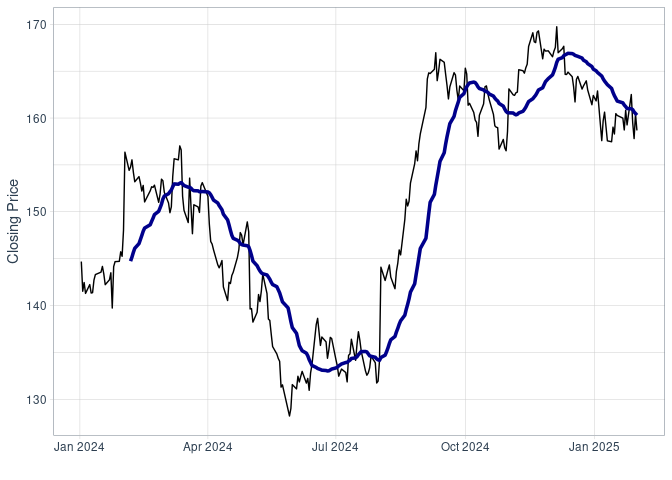
\includegraphics[keepaspectratio]{index_files/figure-latex/notebooks-technical-cell-3-output-1.png}}

By playing with the ``n'' value - the average of the last n-day stock
prices - we produced a line that closely resembles the price line. Since
the SMA line crosses the price line from top to bottom, we're supposed
to anticipate a drop in the stock price.

\textbf{The Bollinger Bands} is another useful tool of technical
analysis. These are ``envelopes plotted at a standard deviation level
above and below a simple moving average of the price'' {[}{``Financial
Modeling with {R}''} (n.d.){]}. They supposed to show the volatility of
a price of the stock and the size of expected change of the price in the
future.

Let's demonstrate.

\begin{Shaded}
\begin{Highlighting}[]
\NormalTok{library(tidyquant)}
\NormalTok{library(ggplot2)}
\NormalTok{library(dplyr)}
\NormalTok{CLX }\OperatorTok{\textless{}{-}}\NormalTok{ tq\_get(}\StringTok{"CLX"}\NormalTok{, get }\OperatorTok{=} \StringTok{"stock.prices"}\NormalTok{, }\ImportTok{from} \OperatorTok{=} \StringTok{"2024{-}01{-}01"}\NormalTok{, }
\NormalTok{               to }\OperatorTok{=} \StringTok{"2025{-}02{-}01"}\NormalTok{)}
\NormalTok{CLX }\OperatorTok{|\textgreater{}}
\NormalTok{  ggplot(aes(x }\OperatorTok{=}\NormalTok{ date, y }\OperatorTok{=}\NormalTok{ close, }\BuiltInTok{open} \OperatorTok{=} \BuiltInTok{open}\NormalTok{,}
\NormalTok{              high }\OperatorTok{=}\NormalTok{ high, low }\OperatorTok{=}\NormalTok{ low, close }\OperatorTok{=}\NormalTok{ close)) }\OperatorTok{+}
\NormalTok{    geom\_line() }\OperatorTok{+}
\NormalTok{    geom\_bbands(ma\_fun }\OperatorTok{=}\NormalTok{ SMA, sd }\OperatorTok{=} \DecValTok{2}\NormalTok{, n }\OperatorTok{=} \DecValTok{25}\NormalTok{,}
\NormalTok{                linetype }\OperatorTok{=} \DecValTok{2}\NormalTok{, size }\OperatorTok{=} \FloatTok{0.5}\NormalTok{, alpha }\OperatorTok{=} \FloatTok{0.2}\NormalTok{,}
\NormalTok{                fill        }\OperatorTok{=}\NormalTok{ palette\_light()[[}\DecValTok{1}\NormalTok{]],}
\NormalTok{                color\_bands }\OperatorTok{=}\NormalTok{ palette\_light()[[}\DecValTok{1}\NormalTok{]],}
\NormalTok{                color\_ma    }\OperatorTok{=}\NormalTok{ palette\_light()[[}\DecValTok{2}\NormalTok{]]) }\OperatorTok{+}
\NormalTok{    labs(y }\OperatorTok{=} \StringTok{"Closing Price"}\NormalTok{, x }\OperatorTok{=} \StringTok{""}\NormalTok{) }\OperatorTok{+}
\NormalTok{    theme\_tq()}
\end{Highlighting}
\end{Shaded}

\pandocbounded{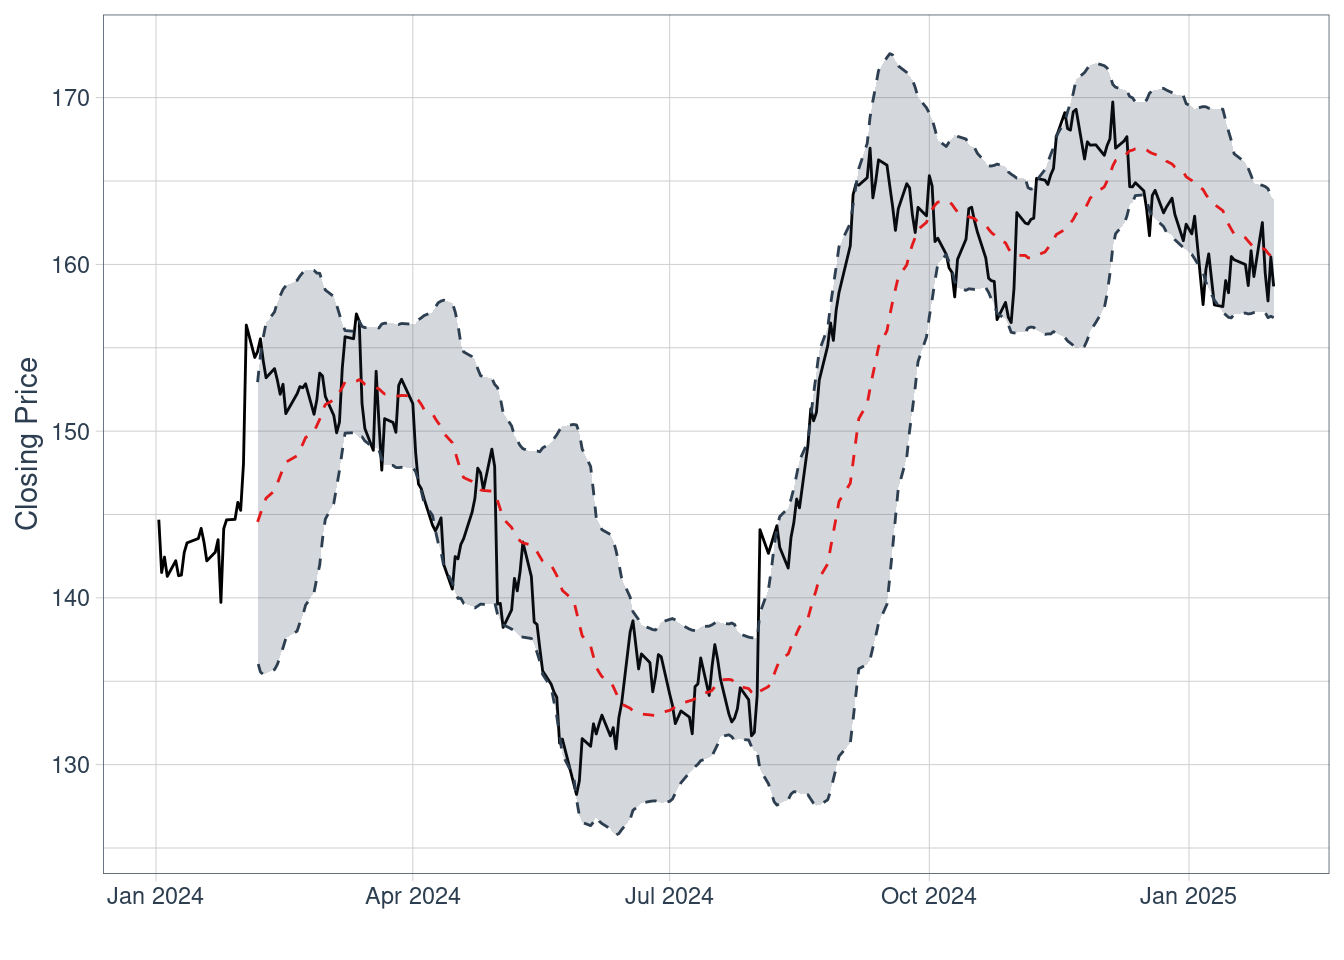
\includegraphics[keepaspectratio]{index_files/figure-latex/notebooks-technical-cell-4-output-2.png}}

And finally let's look at such charts for major competitors to get the
feel of the market.

\begin{Shaded}
\begin{Highlighting}[]
\NormalTok{library(tidyquant)}
\NormalTok{library(ggplot2)}
\NormalTok{library(dplyr)}
\NormalTok{prices }\OperatorTok{\textless{}{-}}\NormalTok{ tq\_get(c(}\StringTok{"CLX"}\NormalTok{, }\StringTok{"CL"}\NormalTok{, }\StringTok{"PG"}\NormalTok{, }\StringTok{"CHD"}\NormalTok{), get }\OperatorTok{=} \StringTok{"stock.prices"}\NormalTok{, }\ImportTok{from} \OperatorTok{=} \StringTok{"2024{-}01{-}01"}\NormalTok{, }
\NormalTok{  to }\OperatorTok{=} \StringTok{"2025{-}02{-}01"}\NormalTok{)}
\NormalTok{prices }\OperatorTok{|\textgreater{}}
\NormalTok{  ggplot(aes(x }\OperatorTok{=}\NormalTok{ date, y }\OperatorTok{=}\NormalTok{ close, }\BuiltInTok{open} \OperatorTok{=} \BuiltInTok{open}\NormalTok{,}
\NormalTok{              high }\OperatorTok{=}\NormalTok{ high, low }\OperatorTok{=}\NormalTok{ low, close }\OperatorTok{=}\NormalTok{ close)) }\OperatorTok{+}
\NormalTok{    geom\_line() }\OperatorTok{+}
\NormalTok{    geom\_bbands(ma\_fun }\OperatorTok{=}\NormalTok{ SMA, sd }\OperatorTok{=} \DecValTok{2}\NormalTok{, n }\OperatorTok{=} \DecValTok{25}\NormalTok{,}
\NormalTok{                linetype }\OperatorTok{=} \DecValTok{2}\NormalTok{, size }\OperatorTok{=} \FloatTok{0.5}\NormalTok{, alpha }\OperatorTok{=} \FloatTok{0.2}\NormalTok{,}
\NormalTok{                fill        }\OperatorTok{=}\NormalTok{ palette\_light()[[}\DecValTok{1}\NormalTok{]],}
\NormalTok{                color\_bands }\OperatorTok{=}\NormalTok{ palette\_light()[[}\DecValTok{1}\NormalTok{]],}
\NormalTok{                color\_ma    }\OperatorTok{=}\NormalTok{ palette\_light()[[}\DecValTok{2}\NormalTok{]]) }\OperatorTok{+}
\NormalTok{    facet\_wrap(}\OperatorTok{\textasciitilde{}}\NormalTok{ symbol, ncol }\OperatorTok{=} \DecValTok{2}\NormalTok{, scales }\OperatorTok{=} \StringTok{"free\_y"}\NormalTok{) }\OperatorTok{+}
\NormalTok{    theme\_tq()}
\end{Highlighting}
\end{Shaded}

\pandocbounded{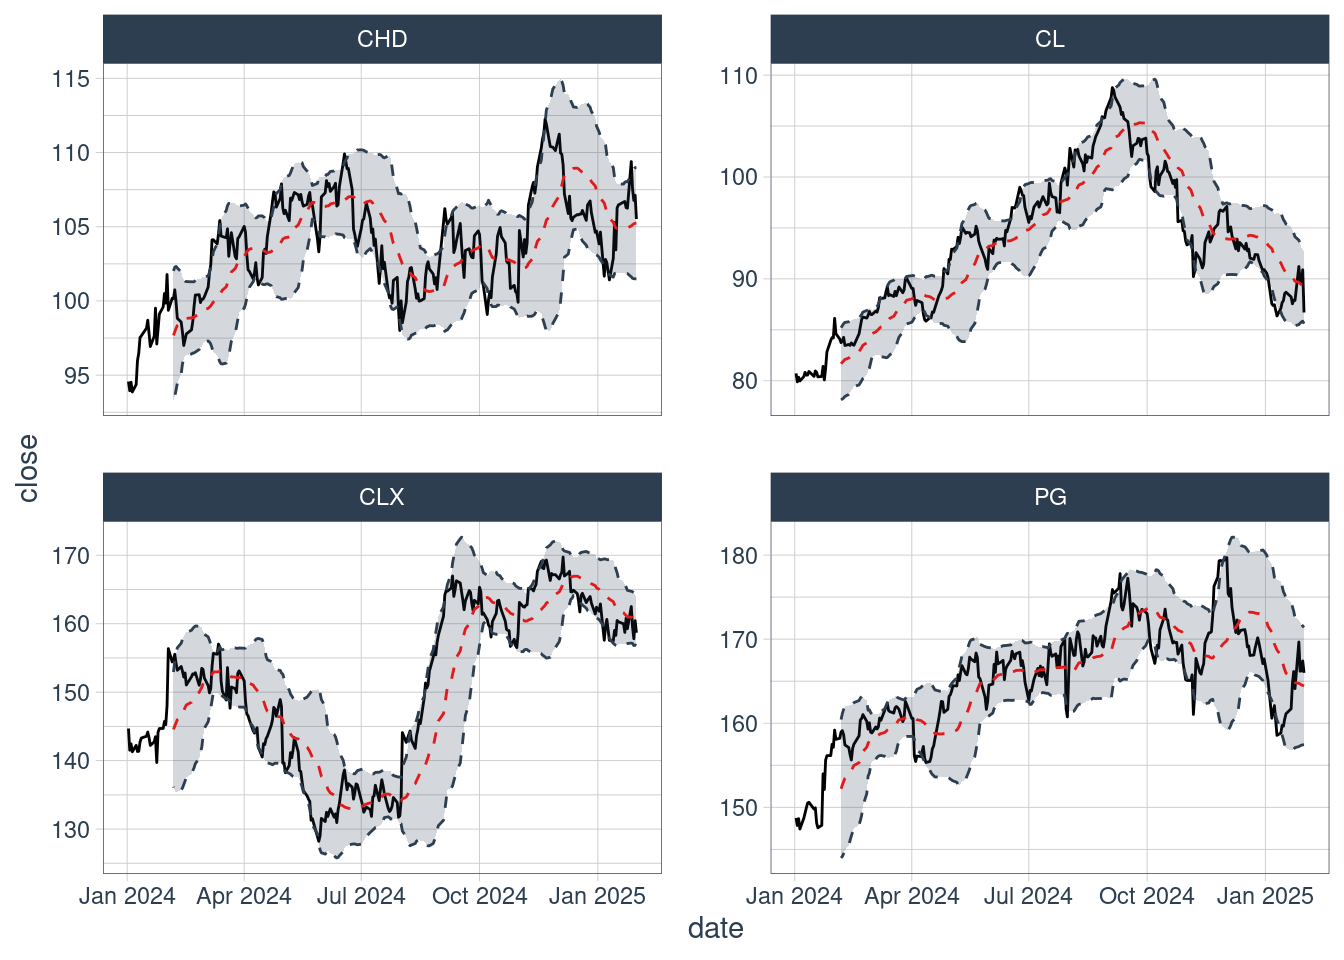
\includegraphics[keepaspectratio]{index_files/figure-latex/notebooks-technical-cell-5-output-2.png}}

As we can see, the volatility of the stock prices shouldn't be that
great in the near future. Since technical analysis is best-suited for
short-term trading, near future is all we can advise or client on based
on such analysis.

\subsubsection{Conclusion}\label{conclusion-3}

We can use ``tidyquant'' R language package along with other packages
for producing charts to perform basic technical analysis of stock price.
The analysis predicts stable performance in the short term.

\subsection{Company Performance
2019-2024}\label{company-performance-2019-2024}

\section{}\label{section-5}

\begin{quote}
\textbf{Note}

In this section we provide some historic data and rudimentary analysis
of the company during the 2019-2024 period.
\end{quote}

\subsubsection{Historical Analysis of the
Company}\label{historical-analysis-of-the-company}

As we've identified in the previous sections, major events for the
company in this peroid included the adoption of IGNITE strategy and
recent cyberattack. Another major event was, of course, the global
pandemic.

In terms of the corporation's life cycle, Clorox is definitely in the
\textbf{Maturity} phase: it is relatively stable, resilient to shocks
and demonstrates confidence during the recovery from such shocks.

Getting historical data is very easy with R language - you just provide
the time period you are interested in, and get it same as always.

\begin{Shaded}
\begin{Highlighting}[]
\NormalTok{library(tidyquant)}
\end{Highlighting}
\end{Shaded}

\pandocbounded{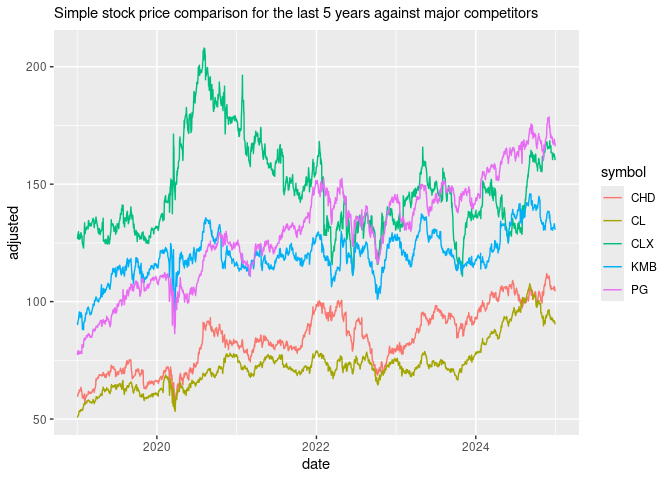
\includegraphics[keepaspectratio]{index_files/figure-latex/notebooks-2019-2024-cell-2-output-2.png}}

Fundamental analysis based on revenue data for the last five-year period
can be found in the ``Fundamental Analysis'' section.

\begin{center}\rule{0.5\linewidth}{0.5pt}\end{center}

Sites like \url{https://stockanalysis.com} provide all kinds of historic
data for the last five-year period in nice tables. All of it can be
scraped - we'll scrape and reproduce some of it here.

\begin{longtable}[]{@{}
  >{\raggedright\arraybackslash}p{(\linewidth - 12\tabcolsep) * \real{0.2208}}
  >{\raggedright\arraybackslash}p{(\linewidth - 12\tabcolsep) * \real{0.1299}}
  >{\raggedright\arraybackslash}p{(\linewidth - 12\tabcolsep) * \real{0.1299}}
  >{\raggedright\arraybackslash}p{(\linewidth - 12\tabcolsep) * \real{0.1299}}
  >{\raggedright\arraybackslash}p{(\linewidth - 12\tabcolsep) * \real{0.1299}}
  >{\raggedright\arraybackslash}p{(\linewidth - 12\tabcolsep) * \real{0.1299}}
  >{\raggedright\arraybackslash}p{(\linewidth - 12\tabcolsep) * \real{0.1299}}@{}}
\toprule\noalign{}
\begin{minipage}[b]{\linewidth}\raggedright
Fiscal Year
\end{minipage} & \begin{minipage}[b]{\linewidth}\raggedright
Current
\end{minipage} & \begin{minipage}[b]{\linewidth}\raggedright
FY 2024
\end{minipage} & \begin{minipage}[b]{\linewidth}\raggedright
FY 2023
\end{minipage} & \begin{minipage}[b]{\linewidth}\raggedright
FY 2022
\end{minipage} & \begin{minipage}[b]{\linewidth}\raggedright
FY 2021
\end{minipage} & \begin{minipage}[b]{\linewidth}\raggedright
FY 2020
\end{minipage} \\
\midrule\noalign{}
\endhead
\bottomrule\noalign{}
\endlastfoot
Period Ending & Feb '25 Feb 14, 2025 & Jun '24 Jun 30, 2024 & Jun '23
Jun 30, 2023 & Jun '22 Jun 30, 2022 & Jun '21 Jun 30, 2021 & Jun '20 Jun
30, 2020 \\
Market Capitalization & 18,222 & 16,948 & 19,661 & 17,352 & 22,376 &
27,626 \\
Market Cap Growth & 13.64\% & -13.80\% & 13.31\% & -22.45\% & -19.00\% &
41.66\% \\
Enterprise Value & 21,024 & 19,913 & 22,613 & 20,467 & 25,241 &
30,412 \\
Last Close Price & 147.92 & 133.25 & 150.09 & 128.86 & 159.95 &
190.95 \\
PE Ratio & 40.32 & 60.53 & 131.95 & 37.56 & 31.52 & 29.42 \\
Forward PE & 20.81 & 21.90 & 29.44 & 28.13 & 25.00 & 30.85 \\
PS Ratio & 2.56 & 2.39 & 2.66 & 2.44 & 3.05 & 4.11 \\
PB Ratio & 166.14 & 34.45 & 50.67 & 23.80 & 37.80 & 30.43 \\
\end{longtable}

CLX's Historical Financial Ratios, source: {``The {Clorox Market} Share
Relative to Its Competitors, as of {Q4} 2024 - {CSIMarket}''} (n.d.)

\subsubsection{Conclusion}\label{conclusion-4}

We can use publicly available data, as well as the R language to get
historical financial data and ratios. The analysis shows strong
performance during the last five-year period.

\subsection{Forecasting}\label{forecasting}

\section{}\label{section-6}

\begin{quote}
\textbf{Note}

In this section we use ARIMA model to provide a long-term forecast of
the company stock price.
\end{quote}

\subsubsection{\texorpdfstring{\textbf{Long-Term Financial Forecast for
the Company Using ARIMA
Model}}{Long-Term Financial Forecast for the Company Using ARIMA Model}}\label{long-term-financial-forecast-for-the-company-using-arima-model}

Long-term financial forecasting, like all social forecasting, is an
incredibly fraught undertaking due to many different reasons (see, for
example, {[}Cerqueira (2022){]} and {[}{``Forecasting and Predictive
Analytics: {A} Critical Look at the Basic Building Blocks of a
Predictive Model''} (n.d.){]}). Luckily, many tools are available for us
to experiment with.

We've already done some simple short-term forecasting in our ``Technical
Analysis'' section using \textbf{SMA} and \textbf{Bollinger Bands}.
We've also accessed volatility by calculating \textbf{Beta} value and
estimated risk/return using \textbf{Annualized Sharpe Ratio}, which
might help us in medium-term forecasting. Now we will try using advanced
\textbf{ARIMA} (Auto-Regressive Integrated Moving Averages) to predict
stock prices for the next 6 months and for the next year.

\begin{Shaded}
\begin{Highlighting}[]
\NormalTok{library(tidyquant)}
\end{Highlighting}
\end{Shaded}

\pandocbounded{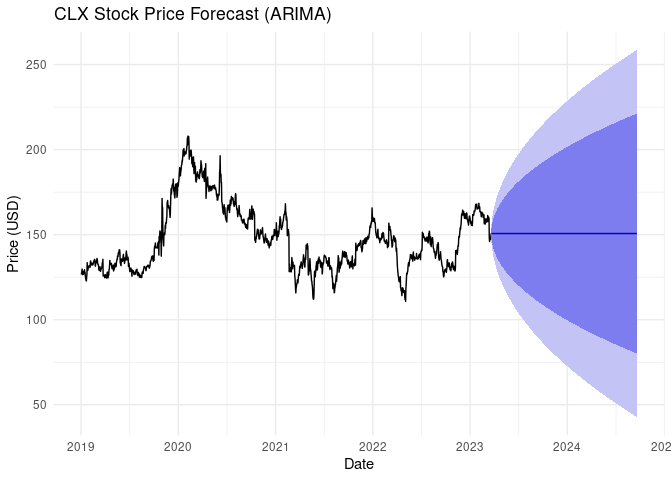
\includegraphics[keepaspectratio]{index_files/figure-latex/notebooks-forecasting-cell-2-output-2.png}}

\pandocbounded{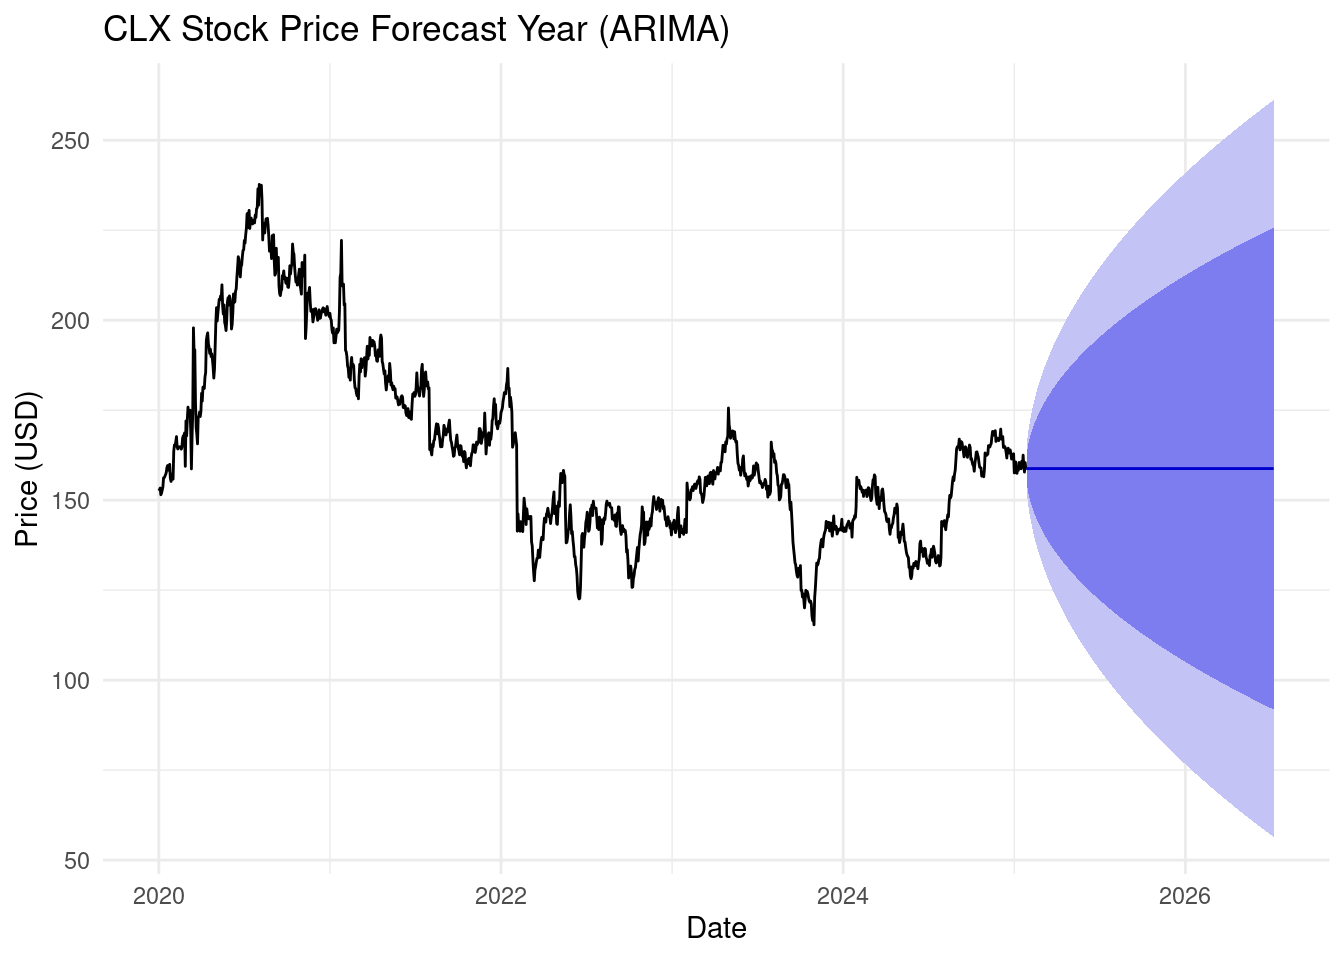
\includegraphics[keepaspectratio]{index_files/figure-latex/notebooks-forecasting-cell-2-output-3.png}}

We can see the band for the future time periods representing possible
price ranges and 2 confidence levels.

\subsubsection{\texorpdfstring{\textbf{Conclusion}}{Conclusion}}\label{conclusion-5}

We can use advanced forecasting models (such as ARIMA) available in the
R language to predict the stock price. The analysis shows a wide range
of possible future prices, albeit without major ups or downs.

\subsection{Summary}\label{summary}

\section{}\label{section-7}

\subsubsection{\texorpdfstring{\textbf{Analysis Summary and Letter
Grade}}{Analysis Summary and Letter Grade}}\label{analysis-summary-and-letter-grade}

Our analysis shows mature company with stable management, good branding,
strong fundamentals and good estimated prospects. We give the letter
grade \textbf{B} for the company and recommend including its stock in
the investment portfolio. Of course, no one single stock should be
recommended individually for investment, but portfolio management is out
of scope for this document.

\subsubsection{\texorpdfstring{\textbf{Advice for the
Fiduciary}}{Advice for the Fiduciary}}\label{advice-for-the-fiduciary}

This document provides the fiduciary with basic tools for the
quantitative analysis of individual corporations. These tools are indeed
\textbf{basic} and should only be viewed as a starting point for serious
analysis. There are many great ways to learn more about finance and
investment. We would recommend to look at the following sources (which
we ourselves used to prepare this document) to learn more:
{[}{``Quantitative Finance with {R}''} (n.d.){]}, {[}Wahlen, Baginski,
and Bradshaw (2022){]}, {[}\emph{Forecasting: {Principles} and
{Practice} (2nd Ed)} (n.d.){]}, {[}{``R for {Data Science} (2e)''}
(n.d.){]}, {[}{``Tidy {Quantitative Financial Analysis}''} (n.d.){]},
{[}{``Investopedia''} (n.d.){]}.

\phantomsection\label{refs}
\begin{CSLReferences}{1}{0}
\bibitem[\citeproctext]{ref-cerqueira8ReasonsWhy2022}
Cerqueira, Vitor. 2022. {``8 {Reasons Why Forecasting Is Hard}.''}
\emph{Towards Data Science}.
https://towardsdatascience.com/8-reasons-why-forecasting-is-hard-481755a05325/.

\bibitem[\citeproctext]{ref-danchoTidyquantTidyQuantitative2025}
Dancho, Matt, and Davis Vaughan. 2025. {``Tidyquant: {Tidy Quantitative
Financial Analysis}.''}

\bibitem[\citeproctext]{ref-FinancialModelingb}
{``Financial Modeling with {R}.''} n.d.
https://mlozanoqf.github.io/tutorial\_pmf/. Accessed February 14, 2025.

\bibitem[\citeproctext]{ref-ForecastingPredictiveAnalytics}
{``Forecasting and Predictive Analytics: {A} Critical Look at the Basic
Building Blocks of a Predictive Model.''} n.d. \emph{Brookings}.
https://www.brookings.edu/articles/forecasting-and-predictive-analytics-a-critical-look-at-the-basic-building-blocks-of-a-predictive-model/.
Accessed February 15, 2025.

\bibitem[\citeproctext]{ref-ForecastingPrinciplesPractice}
\emph{Forecasting: {Principles} and {Practice} (2nd Ed)}. n.d. Accessed
February 15, 2025.

\bibitem[\citeproctext]{ref-IGNITEStrategy}
{``{IGNITE Strategy}.''} n.d. \emph{The Clorox Company}. Accessed
February 14, 2025.

\bibitem[\citeproctext]{ref-Investopedia}
{``Investopedia.''} n.d. \emph{Investopedia}.
https://www.investopedia.com/. Accessed February 15, 2025.

\bibitem[\citeproctext]{ref-mascellinoCloroxOperationsDisrupted2023}
Mascellino, Alessandro. 2023. {``Clorox {Operations Disrupted By
Cyber-Attack}.''} \emph{Infosecurity Magazine}.
https://www.infosecurity-magazine.com/news/clorox-disrupted-cyber-attack/.

\bibitem[\citeproctext]{ref-PerformanceAnalysisTidyquant}
{``Performance {Analysis} with Tidyquant.''} n.d.
https://business-science.github.io/tidyquant/articles/TQ05-performance-analysis-with-tidyquant.html.
Accessed February 14, 2025.

\bibitem[\citeproctext]{ref-PurposeValues}
{``Purpose \& {Values}.''} n.d. \emph{The Clorox Company}. Accessed
February 14, 2025.

\bibitem[\citeproctext]{ref-QuantitativeFinancea}
{``Quantitative Finance with {R}.''} n.d. https://mlozanoqf.github.io/.
Accessed February 15, 2025.

\bibitem[\citeproctext]{ref-Quarto}
{``Quarto.''} n.d. \emph{Quarto}. https://quarto.org/. Accessed February
14, 2025.

\bibitem[\citeproctext]{ref-DataScience2e}
{``R for {Data Science} (2e).''} n.d. https://r4ds.hadley.nz/. Accessed
February 11, 2025.

\bibitem[\citeproctext]{ref-ProjectStatisticalComputing}
{``R: {The R Project} for {Statistical Computing}.''} n.d.
https://www.r-project.org/. Accessed February 14, 2025.

\bibitem[\citeproctext]{ref-Recognitions}
{``Recognitions.''} n.d. \emph{The Clorox Company}. Accessed February
14, 2025.

\bibitem[\citeproctext]{ref-Responsibility}
{``Responsibility.''} n.d. \emph{The Clorox Company}. Accessed February
14, 2025.

\bibitem[\citeproctext]{ref-CloroxCompanyCLX}
{``The {Clorox Company} ({CLX}) {Company Profile} \& {Facts}.''} n.d.
\emph{Yahoo Finance}. https://finance.yahoo.com/quote/CLX/profile/.
Accessed February 13, 2025.

\bibitem[\citeproctext]{ref-CloroxCompanyCLXa}
{``The {Clorox Company} ({CLX}) {Leadership} \& {Management Team
Analysis}.''} n.d. \emph{Simply Wall St}.
https://simplywall.st/stocks/us/household/nyse-clx/clorox/management.
Accessed February 14, 2025.

\bibitem[\citeproctext]{ref-CloroxCompanyBusiness}
{``The {Clorox Company}: {Business Model}, {SWOT Analysis}, and
{Competitors} 2024 - {PitchGrade}.''} n.d.
https://pitchgrade.com/companies/the-clorox-company. Accessed February
13, 2025.

\bibitem[\citeproctext]{ref-CloroxMarketShare}
{``The {Clorox Market} Share Relative to Its Competitors, as of {Q4}
2024 - {CSIMarket}.''} n.d.
https://csimarket.com/stocks/competitionSEG2.php?code=CLX. Accessed
February 14, 2025.

\bibitem[\citeproctext]{ref-TidyQuantitativeFinancial}
{``Tidy {Quantitative Financial Analysis}.''} n.d.
https://business-science.github.io/tidyquant/. Accessed February 13,
2025.

\bibitem[\citeproctext]{ref-wahlenFinancialReportingFinancial2022}
Wahlen, James M., Stephen P. Baginski, and Mark Bradshaw. 2022.
\emph{Financial Reporting, Financial Statement Analysis, and Valuation:
A Strategic Perspective}. 10. ed. Boston, MA: Cengage.

\end{CSLReferences}




\end{document}
